% La derivada como aproximación lineal: jacobiano, gradiente y hessiana
% Números del texto nuevo verificados con apunte/scripts/cap10_derivada_jacobiano.py
\chapter{La derivada como aproximación lineal: jacobiano, gradiente y hessiana}\label{cap:derivada}

\section{La idea}

Imaginá que mirás un mapa de rutas con una lupa. Elegís un punto sobre una ruta que serpentea
entre las sierras y vas cambiando a lupas cada vez más potentes. ¿Qué ves? Las curvas se abren,
y con suficiente aumento el tramo que queda en el vidrio parece una recta. No es que la ruta
sea recta: mirada de muy cerca, cualquier curva suave se confunde con una recta, y de esa recta
alcanza con saber por dónde pasa y con qué inclinación. Esa recta es la derivada. La derivada es
la mejor manera de reemplazar, cerca de un punto, una función curva por una función lineal, y
para eso sirve: lo curvo es difícil de calcular, y lo lineal lo sabemos manejar con todo lo que
vimos de matrices.

Pensá ahora en un temblor de la mano al apuntar. Desde un punto conocido apuntás a otro que
está a un kilómetro y medís hacia dónde está y a qué distancia. Si la dirección se corre una
fracción de grado, ¿cuánto se corre el punto que calculás? La cuenta que lleva de lo medido al
punto es curva (tiene senos y cosenos), pero el corrimiento es chico, y para corrimientos
chicos la respuesta es una matriz por un vector. El capítulo construye esa matriz y la usa al
final del capítulo para contestar la pregunta.

El capítulo~\ref{cap:cambio-base} cerró anotando que la métrica \(J^TJ\) de una
parametrización cambia por congruencia; ahora construimos ese \(J\), la matriz que dice
cuánto se estira y hacia dónde gira cada dirección cerca de un punto. Llamamos \emph{pasito} a
cuánto nos corremos desde el punto de partida: un número en la recta, una flecha en el plano o
en el espacio. Subimos la escalera de a un peldaño: la recta, el plano, cualquier dimensión. En
los tres la frase es la misma: \emph{la derivada es lo que multiplica al pasito}; cambia qué
tipo de objeto multiplica.

\paragraph{En \(\R\): un número.} ¿Cuánto da \(\sqrt{100{,}5}\) sin calculadora? Sabemos que la
raíz de \(100\) es \(10\) y que medio punto más arriba la raíz crece un poco. Cuánto, lo dice la
derivada \(f'(x)\), la inclinación de la recta que ve la lupa en \(x\). Si \(f\) es derivable en
\(x\) y \(h\) es el pasito,
\[
  f(x+h)\approx f(x)+f'(x)\,h .
\]
Con \(f(x)=\sqrt x\) en \(x=100\), \(f'(100)=\tfrac1{20}\), y el pasito \(h=0{,}5\) da
\(\sqrt{100{,}5}\approx10+0{,}5/20=10{,}025\); el valor exacto es \(10{,}024969\). La
derivada es una matriz de \(1\times1\): multiplica el pasito por \(\tfrac1{20}\).

\paragraph{En \(\R^n\to\R\): una fila.} Imaginá que estás parado en una ladera y das un paso
corto. ¿Cuánto subiste? Depende de hacia dónde diste el paso: hacia la cumbre, bastante; a lo
largo de la ladera, nada; hacia abajo, una cantidad negativa. Ahora la función toma un punto
del plano y devuelve un número (la altura del terreno, una temperatura), y el pasito es una
columna \(v\), con una componente \(v_x\) en la dirección \(x\) y otra \(v_y\) en la dirección
\(y\). Alcanza con conocer la pendiente en esas dos direcciones, como si apoyáramos una regla
corta en el suelo primero en una y después en la otra, para saber cuánto se sube en cualquier
otra. Esas dos pendientes son las derivadas parciales \(\partial_xf\) y \(\partial_yf\), cuánto
cambia \(f\) por cada unidad que nos movemos solo en \(x\) o solo en \(y\), y puestas en fila
forman el \emph{gradiente}, la fila que multiplica al pasito:
\[
  f(p+v)\approx f(p)+\begin{pmatrix}\partial_xf&\partial_yf\end{pmatrix}
  \begin{pmatrix}v_x\\v_y\end{pmatrix}.
\]
Con \(f(x,y)=x^2y\) en \(p=(1,2)\) la fila es \((2xy,\ x^2)=(4,1)\), y el pasito
\(v=(0{,}1;\ -0{,}1)\) da \(4\cdot0{,}1-1\cdot0{,}1=0{,}3\) contra un cambio real de
\(0{,}299\). Que esa fila sea una forma lineal y no una flecha se vio en la
sección~\ref{sec:gradiente-forma}.

\paragraph{En \(\R^n\to\R^m\): una matriz.} Suponé ahora que la función no devuelve un número
sino varios: un punto del plano, o una distancia y una dirección. Cada componente tiene su
fila, y apiladas forman una matriz, el \emph{jacobiano} \(J\):
\[
  F(p+v)\approx F(p)+J\,v .
\]
La definición precisa dice qué significa el \enquote{\(\approx\)}: lo que la aproximación deja
afuera se achica más rápido que el pasito. Eso se escribe \(\operatorname{o}(\lVert v\rVert)\),
que se lee \enquote{o chica de la norma de \(v\)}: un error que, dividido por el largo del
pasito, tiende a cero. En el enunciado, \(U\) es la región donde está definida \(F\); que sea
abierta quiere decir que alrededor de cada uno de sus puntos hay lugar para dar pasitos en
todas las direcciones.

\begin{definicion}[Diferencial y jacobiano]\label{def:jacobiano}
Sea \(F\colon U\subset\R^n\to\R^m\), con \(U\) abierto, y \(p\in U\). Decimos que \(F\) es
\emph{diferenciable} en \(p\) si existe una matriz \(J\) de \(m\times n\) tal que
\[
  F(p+v)=F(p)+J\,v+\operatorname{o}(\lVert v\rVert),
\]
es decir, el error dividido por \(\lVert v\rVert\) tiende a \(0\) cuando \(v\to0\). La
transformación lineal \(v\mapsto Jv\) es el \emph{diferencial} \(dF_p\) y la matriz \(J=J_F(p)\)
es el \emph{jacobiano}: su fila \(i\) es el gradiente de la componente \(F_i\) y su columna
\(j\) es la derivada parcial \(\partial F/\partial x_j\), la imagen del \(j\)-ésimo vector de la
base.
\end{definicion}

El diferencial \(dF_p\) es la transformación lineal que imita a \(F\) cerca de \(p\); el
jacobiano es la matriz que la escribe en coordenadas. Es la misma diferencia que hay entre una
transformación y su matriz.

\begin{idea}[La derivada es la matriz que mejor imita a la función cerca del punto]
Con una lupa cada vez más potente, una función diferenciable se vuelve indistinguible de
\(v\mapsto Jv\). Todo lo que sabemos de matrices (determinante, inversa, autovalores) se usa
entonces, localmente, sobre funciones que no son lineales.
\end{idea}

\unidadInteractiva{10_jacobiano_primera_forma}{Jacobiano y primera forma fundamental}{Explorá: con la superficie «la loma», poné el punto en la ladera \((2,1)\) y agrandá de a poco el pasito \((du,dv)\). Mirá cuándo el segmento punteado \(J\,(du,dv)\) se separa del pasito curvo sobre la superficie y cuándo la longitud por fórmula deja de coincidir con la de la cinta.}

\subsection{Pasar del plano a una superficie}\label{sec:plano-superficie}

¿Cómo se mide una distancia sobre una loma? Imaginá que caminás por ella con una cinta
métrica. En cada lugar, el suelo bajo tus pies parece un plano un poco inclinado, pero la
inclinación cambia a medida que avanzás. Sobre una superficie curva no existe una única base
cartesiana válida en todas partes. En cada punto aparece un plano tangente, el plano que la
lupa ve en ese punto, y una base local que cambia al desplazarse. Si ubicamos los puntos de la
superficie con dos números \(u\) y \(v\), un pasito \((du,dv)\) es un cambio chico de esos dos
números, y la métrica \(ds^2=E\,du^2+2F\,du\,dv+G\,dv^2\) (sección~\ref{sec:metrica}), con tres
coeficientes \(E\), \(F\), \(G\) que hacen de cinta métrica en cada lugar, convierte esos
pequeños cambios de coordenadas en distancias sobre la superficie.

\begin{idea}[De lo global a lo local]
Una superficie curva se estudia con pequeños parches que se parecen a un plano, cada uno con
sus coordenadas locales: es la intuición de una variedad (sección~\ref{sec:variedades}).
\end{idea}

\begin{idea}[La derivada como mejor aproximación lineal]
El gradiente es perpendicular a una curva o superficie de nivel porque es una forma lineal: la
curva de nivel \(0\) de esa forma es la recta (o el plano) tangente.
\end{idea}

\section{Construcciones, cuentas y ejemplos}


\subsection{El jacobiano: la matriz de la aproximación}\label{sec:jacobiano}

Imaginá una lámina de goma con una cuadrícula dibujada, y que alguien la estira de manera
despareja, más en un lado que en otro. ¿En qué se convierte una celda chiquita? Mirada con la
lupa, en un paralelogramo, y ese paralelogramo lo dan las columnas de \(J\). Para armar \(J\)
hay dos lecturas, las mismas que en cualquier matriz. Por filas: cada componente de \(F\) es una
función a valores reales y su fila es su gradiente, una forma lineal que mide cuánto cambia esa
componente. Por columnas: la columna \(j\) es la velocidad con que se mueve \(F(p)\) cuando solo
cambia la coordenada \(x_j\): el vector tangente a la imagen de la línea coordenada \(j\). En la
cuadrícula, las columnas de \(J\) son los lados del paralelogramo en que se transforma una celda
chiquita; por eso su determinante es el factor local de área, el número por el que se
multiplica el área de una celda chica (proposición~\ref{prop:det-factor} del
capítulo~\ref{cap:subespacios}).

Las coordenadas polares son el primer caso. En ellas un punto se da con su distancia \(r\) al
origen y con el ángulo \(\theta\) que forma con el eje \(x\), y la función \(P\) del ejemplo
convierte ese par en las coordenadas cartesianas del punto.

\begin{ejemplo}[Jacobiano de polares a cartesianas]\label{ej:der-polares}
Sea \(P(r,\theta)=(r\cos\theta,\ r\sin\theta)\). Derivando cada componente respecto de \(r\) y
de \(\theta\),
\[
  J_P(r,\theta)=\begin{pmatrix}\cos\theta&-r\sin\theta\\ \sin\theta&r\cos\theta\end{pmatrix},
  \qquad \det J_P=r\cos^2\theta+r\sin^2\theta=r .
\]
En \(r=2\), \(\theta=30^\circ\) el punto es \(P=(1{,}732;\ 1)\) y
\[
  J=\begin{pmatrix}0{,}866&-1\\0{,}5&1{,}732\end{pmatrix},\qquad \det J=2 .
\]
La primera columna, \((0{,}866;\ 0{,}5)\), es el versor radial: avanzar en \(r\) es alejarse
del origen a lo largo del rayo. La segunda, \((-1;\ 1{,}732)\), es perpendicular a la primera y
mide \(r=2\): girar un radián desplaza el punto dos unidades a lo largo de la circunferencia.

Tomamos el rectangulito \(dr=0{,}1\), \(d\theta=0{,}05\) rad del plano \((r,\theta)\) con
esquina en \((2,30^\circ)\) y comparamos la imagen exacta de sus vértices con la que predice
\(J\) (desplazamientos desde \(P(2,30^\circ)\)):
\begin{center}
\begin{tabular}{lccc}
pasito & imagen exacta & \(J\,(dr,d\theta)\) & diferencia\\\hline
\((0{,}1;\ 0)\) & \((0{,}0866;\ 0{,}05)\) & \((0{,}0866;\ 0{,}05)\) & \(0\)\\
\((0;\ 0{,}05)\) & \((-0{,}0521;\ 0{,}0853)\) & \((-0{,}05;\ 0{,}0866)\) & \(0{,}0025\)\\
\((0{,}1;\ 0{,}05)\) & \((0{,}0319;\ 0{,}1396)\) & \((0{,}0366;\ 0{,}1366)\) & \(0{,}0056\)
\end{tabular}
\end{center}
El lado radial coincide exactamente porque los rayos son rectas; el lado en \(\theta\) es un
arco, y su cuerda se aparta de la tangente en un término de segundo orden. El área exacta de
la celda imagen (un trapecio polar) es
\(\tfrac12\,d\theta\,\bigl((r+dr)^2-r^2\bigr)=0{,}01025\), y la que da el jacobiano es
\(\lvert\det J\rvert\,dr\,d\theta=r\,dr\,d\theta=0{,}01\). La diferencia, \(0{,}00025\), es
\(\tfrac12\,dr^2\,d\theta\): de orden superior. Es el origen del factor \(r\) en
\(dA=r\,dr\,d\theta\), y del cambio de variables en las integrales dobles.

Hecho geométrico (figura~\ref{fig:der-polar}): la grilla recta del plano \((r,\theta)\) se
convierte en la grilla de circunferencias y rayos; cada celda chica se ve como el
paralelogramo de lados \(J(dr,0)\) y \(J(0,d\theta)\), que acá es un rectángulo porque las
columnas de \(J\) son perpendiculares, y su área es \(r\) veces la de la celda original.
\end{ejemplo}

\begin{figure}[htbp]
\centering
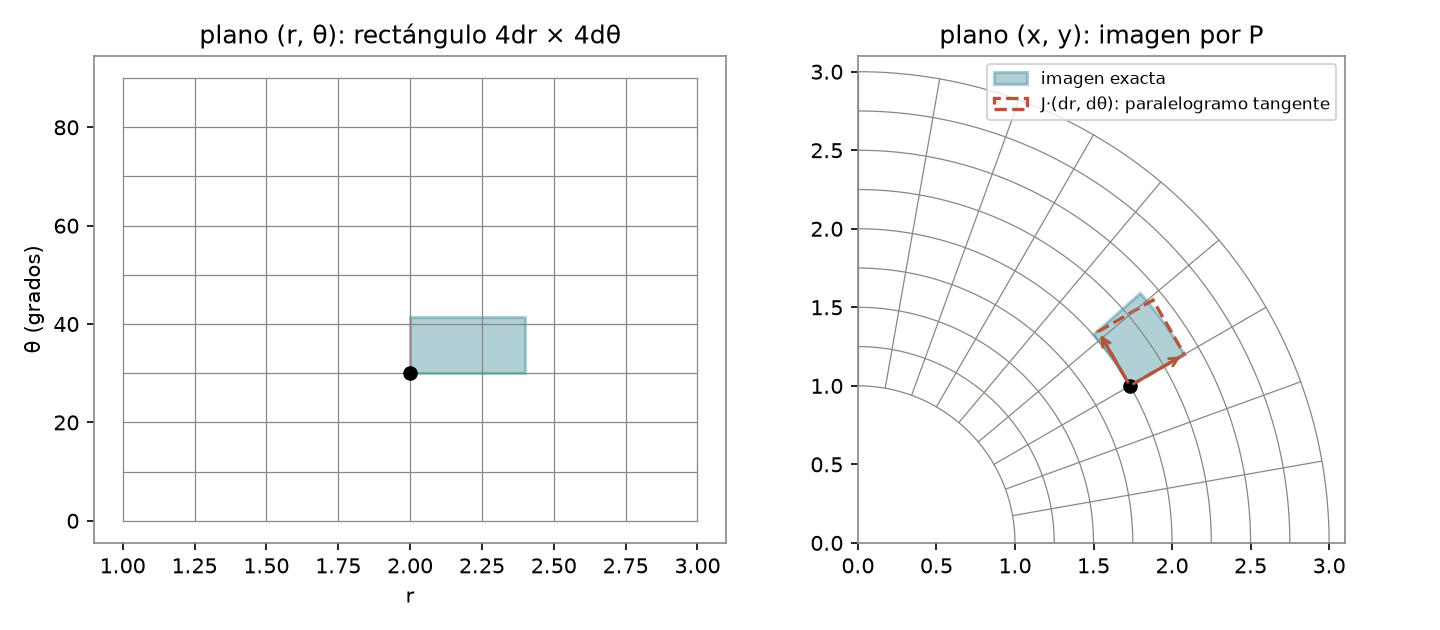
\includegraphics[width=.95\linewidth]{figuras/derivada/der_polar.png}
\caption{Izquierda: un rectángulo del plano \((r,\theta)\) con esquina en \((2,30^\circ)\),
dibujado cuatro veces más grande que el del ejemplo~\ref{ej:der-polares} para que se vea.
Derecha: su imagen exacta por \(P(r,\theta)=(r\cos\theta,r\sin\theta)\) (teal) y el
paralelogramo tangente \(J\,(dr,d\theta)\) (óxido, punteado), cuyos lados son las columnas de
\(J\) escaladas por \(dr\) y \(d\theta\).}
\label{fig:der-polar}
\end{figure}

\subsection{Regla de la cadena: componer es multiplicar}\label{sec:regla-cadena}

Imaginá dos lupas puestas una detrás de la otra: la primera agranda tres veces y la segunda,
dos. ¿Cuánto agranda el conjunto? Seis veces: los aumentos se multiplican. Con funciones pasa lo
mismo. Llamamos \(G\circ F\) a la función que aplica primero \(F\) y después \(G\), cada una con
su jacobiano, \(J_F\) y \(J_G\). Si primero aplicamos \(F\) y después \(G\), los pasitos se
multiplican primero por \(J_F\) y después por \(J_G\): la aproximación lineal de la composición
es el producto de las matrices.

\begin{proposicion}[Regla de la cadena]\label{prop:regla-cadena}
Si \(F\colon\R^n\to\R^m\) es diferenciable en \(p\) y \(G\colon\R^m\to\R^k\) es diferenciable
en \(F(p)\), entonces \(G\circ F\) es diferenciable en \(p\) y
\[
  J_{G\circ F}(p)=J_G\bigl(F(p)\bigr)\,J_F(p) .
\]
\end{proposicion}

\begin{demostracion}
Escribimos \(F(p+v)=F(p)+w\) con \(w=J_Fv+\operatorname{o}(\lVert v\rVert)\); en particular
\(\lVert w\rVert\le C\lVert v\rVert\) para \(v\) chico. Entonces
\(G(F(p+v))=G(F(p))+J_Gw+\operatorname{o}(\lVert w\rVert)
=G(F(p))+J_GJ_Fv+J_G\operatorname{o}(\lVert v\rVert)+\operatorname{o}(\lVert v\rVert)\), y los
dos últimos términos son \(\operatorname{o}(\lVert v\rVert)\).
\end{demostracion}

En \(\R\) es la regla conocida, \((g\circ f)'=g'(f(x))\,f'(x)\): un producto de dos números,
como el de las dos lupas.
Con una función a valores reales al final, es una fila por una matriz, la regla
\enquote{la forma se transforma del lado contrario que el vector} del
capítulo~\ref{cap:formas-lineales}:
si \(h\) da la altura del terreno en función de \((x,y)\) y \((x,y)=P(r,\theta)\), la fila de
\(h\circ P\) es \(dh\,J_P\), donde \(dh\) es la fila de \(h\) (ejercicio~\ref{ex:der-cadena}).

\subsection{La inversa local: el jacobiano de la inversa es la inversa del jacobiano}\label{sec:inversa-local}

Si al pasar por una función una celda chica se estira al doble en una dirección, ¿qué hay que
hacer para volver? Encogerla a la mitad en esa misma dirección. Deshacer una función cerca de un
punto es deshacer su matriz. Si \(F\) tiene una inversa diferenciable \(F^{-1}\), la función
que devuelve cada punto a donde estaba, la regla de la cadena aplicada a
\(F^{-1}\circ F=\mathrm{id}\) (\(\mathrm{id}\) es la función que no mueve nada, y su jacobiano
es la identidad \(I\)) da \(J_{F^{-1}}(F(p))\,J_F(p)=I\): el jacobiano de la inversa
es la inversa del jacobiano. En particular \(\det J_F(p)\neq0\). La recíproca, que no
demostramos acá, es la que da sentido local a todo el capítulo.

\begin{resultado}[Teorema de la función inversa (resultado usado)]
Si \(F\colon\R^n\to\R^n\) tiene derivadas parciales continuas y \(\det J_F(p)\neq0\), entonces
cerca de \(p\) la función \(F\) es invertible, su inversa es diferenciable y
\(J_{F^{-1}}(F(p))=J_F(p)^{-1}\).
\end{resultado}

Es la versión local de lo que el capítulo~\ref{cap:inversas} hace con matrices: donde el
jacobiano se puede invertir, la función se puede deshacer cerca del punto, aunque globalmente
no sea inyectiva (las polares, con \(\det J_P=r\), se pueden invertir cerca de cualquier punto
salvo el origen, pero no en todo el plano, porque \(\theta\) y \(\theta+2\pi\) dan el mismo
punto).

Una situación de campo muestra a la vez el jacobiano y su inversa. Imaginá que estás parado en
un punto de coordenadas conocidas y apuntás a otro. Hay instrumentos que miden ángulos
horizontales con precisión de hasta un segundo de arco y distancias al milímetro: con ellos
sabés hacia dónde está el otro punto y a qué distancia. ¿Cómo se pasa de esos dos números a sus
coordenadas, y de las coordenadas a esos dos números? Son dos funciones, una inversa de la otra,
y sus jacobianos tienen que ser matrices inversas. En el ejemplo, \(E\) y \(N\) son las
coordenadas este y norte, \(d\) es la distancia, \(\mathrm{Az}\) el ángulo respecto del norte, y
\(\operatorname{atan2}\) es la versión del arco tangente que mira los signos de las dos
diferencias para decidir en qué cuadrante cae el ángulo.

\begin{idea}[Esto lo vas a usar en Topografía]
El punto desde donde se mide se llama \emph{estación}. La dirección hacia el otro punto se da
con el \emph{acimut}: el ángulo que forma con el norte, contado en sentido horario, como las
agujas del reloj. Calcular las coordenadas de un punto a partir de la distancia y esa dirección,
medidas desde un punto conocido, se llama \emph{radiación}.
\end{idea}

\begin{ejemplo}[Distancia y acimut desde una estación, y su inversa]\label{ej:der-dist-acimut}
Desde una estación \(S=(E_0,N_0)\), a cada punto \((E,N)\) le asignamos su distancia y su
acimut: con \(\Delta E=E-E_0\), \(\Delta N=N-N_0\),
\[
  \operatorname{Pol}(E,N)=(d,\mathrm{Az}),\qquad d=\sqrt{\Delta E^2+\Delta N^2},\qquad
  \mathrm{Az}=\operatorname{atan2}(\Delta E,\Delta N),
\]
con el acimut medido desde el norte en sentido horario (sección~\ref{sec:acimut-campo}) y en
radianes. Derivando,
\[
  J_{\operatorname{Pol}}=\begin{pmatrix}\dfrac{\Delta E}{d}&\dfrac{\Delta N}{d}\\[2mm]
  \dfrac{\Delta N}{d^2}&-\dfrac{\Delta E}{d^2}\end{pmatrix}
  =\begin{pmatrix}\sin\mathrm{Az}&\cos\mathrm{Az}\\[1mm]
  \dfrac{\cos\mathrm{Az}}{d}&-\dfrac{\sin\mathrm{Az}}{d}\end{pmatrix},
  \qquad \det J_{\operatorname{Pol}}=-\frac1d .
\]
La primera fila es el versor que va de la estación al punto: la distancia solo cambia si nos
movemos en esa dirección. La segunda fila es perpendicular y está dividida por \(d\): el mismo
desplazamiento lateral cambia menos el acimut cuanto más lejos está el punto.

La inversa es la radiación, \(\operatorname{Rad}(d,\mathrm{Az})=(E_0+d\sin\mathrm{Az},\ N_0+d\cos\mathrm{Az})\),
con
\[
  J_{\operatorname{Rad}}=\begin{pmatrix}\sin\mathrm{Az}&d\cos\mathrm{Az}\\ \cos\mathrm{Az}&-d\sin\mathrm{Az}\end{pmatrix}.
\]
Con \(\Delta E=300\) m, \(\Delta N=400\) m resulta \(d=500\) m, \(\mathrm{Az}=36{,}8699^\circ\), y
\[
  J_{\operatorname{Pol}}=\begin{pmatrix}0{,}6&0{,}8\\0{,}0016&-0{,}0012\end{pmatrix},\qquad
  J_{\operatorname{Rad}}=\begin{pmatrix}0{,}6&400\\0{,}8&-300\end{pmatrix},\qquad
  J_{\operatorname{Pol}}J_{\operatorname{Rad}}=\begin{pmatrix}1&0\\0&1\end{pmatrix}.
\]
(A mano: \(0{,}6\cdot0{,}6+0{,}8\cdot0{,}8=1\) y \(0{,}6\cdot400-0{,}8\cdot300=0\).) Las
unidades acompañan: la segunda fila de \(J_{\operatorname{Pol}}\) está en
radianes por metro y la segunda columna de \(J_{\operatorname{Rad}}\) en metros por radián.

Si el punto se corre \((0{,}10;\ -0{,}05)\) m, la aproximación lineal da
\(\Delta d=0{,}6\cdot0{,}10-0{,}8\cdot0{,}05=0{,}02\) m y
\(\Delta\mathrm{Az}=0{,}0016\cdot0{,}10+0{,}0012\cdot0{,}05=0{,}00022\) rad, o sea
\(45{,}38''\). Recalculando con las fórmulas exactas se obtiene \(\Delta d=0{,}02001\) m y
\(45{,}38''\): a esta escala la aproximación lineal es, en la práctica, exacta.
\end{ejemplo}


\subsection{Coordenadas curvilíneas y bases locales}\label{sec:curvilineas}

Imaginá que tenés que ubicar puntos sobre una loma y no sobre un plano. Podés usar dos números,
como en el plano, pero las líneas en que uno de los dos queda fijo ya no son rectas: se curvan
con el terreno. ¿Qué hace de base en cada punto? Una parametrización
\(r\colon U\subset\R^2\to\R^3\), \((u,v)\mapsto r(u,v)\), es una función que a cada par de
números \((u,v)\) de una región \(U\) del plano le asigna un punto \(r(u,v)\) del espacio, y
así describe una superficie mediante dos coordenadas. Los vectores \(r_u=\partial r/\partial u\)
y \(r_v=\partial r/\partial v\), las velocidades con que se mueve el punto cuando cambia solo
\(u\) o solo \(v\), forman una base tangente local cuando son linealmente independientes. En el
dibujo, \(n\) es la normal: la flecha perpendicular a la superficie en \(p\).

\begin{center}
\begin{tikzpicture}[scale=.9]
  \draw[teallight,fill=teallight!60] (1,1)
    .. controls (3,.2) and (6,.5) .. (8,1.4)
    .. controls (7,3.8) and (3.2,4.5) .. (1,3)
    .. controls (.7,2.2) and (.7,1.6) .. cycle;
  \coordinate (p) at (4.6,2.1);
  \fill[ink] (p) circle (2.5pt) node[below left] {$p$};
  \draw[mainline,-{Latex[length=2.6mm]}] (p)--++(2.2,.25)
    node[right] {$r_u$};
  \draw[rust,line width=1.05pt,-{Latex[length=2.6mm]}] (p)--++(-.6,1.7)
    node[above] {$r_v$};
  \draw[muted,line width=.8pt,-{Latex[length=2.6mm]}] (p)--++(.2,2.2)
    node[above] {$n$};
  \node[text=muted] at (6.8,.8) {superficie};
\end{tikzpicture}
\end{center}

En una superficie curva, a diferencia del plano cartesiano, la base cambia de orientación y de
longitud con el punto; por eso los productos internos y las derivadas adquieren coeficientes.

\subsection{Variedades y espacio tangente}\label{sec:variedades}

Pensá en la Tierra: desde donde estás parado el suelo parece plano, y lo curvo aparece recién
cuando se mira lejos. ¿Qué objetos se comportan así? Una variedad es un objeto que localmente
se parece a un espacio euclídeo. Una superficie regular \(S\subset\R^3\), sin pliegues ni puntas, tiene en cada punto
\(p\) un espacio tangente \(T_pS=\operatorname{span}\{r_u(p),r_v(p)\}\), el conjunto de todas
las combinaciones de \(r_u\) y \(r_v\): las flechas que salen de \(p\) rozando la superficie, la
mejor aproximación lineal local a la superficie. Es el plano que ve la lupa. No es una
proyección cartográfica: pertenece al punto \(p\) y cambia al desplazarse sobre \(S\). Si
\(\Phi\colon S\to\mathcal N\) es una aplicación entre superficies (variedades), una regla que
lleva cada punto de \(S\) a un punto de otra superficie \(\mathcal N\), como un mapa que lleva
la Tierra al papel, su derivada \(d\Phi_p\colon T_pS\to T_{\Phi(p)}\mathcal N\) es una
transformación lineal entre espacios tangentes, que contiene la información local sobre
escala, orientación, deformación angular y deformación de áreas.

\subsection{Métrica y primera forma fundamental}\label{sec:metrica}

¿Cuánto mide un pasito \((du,dv)\) sobre la superficie? En el plano cartesiano la respuesta es
Pitágoras. Sobre una loma, las flechas \(r_u\) y \(r_v\) no miden uno ni son perpendiculares, y
Pitágoras necesita una corrección. La métrica inducida por la parametrización, la cinta métrica
de cada lugar, queda determinada por tres productos internos (\(\langle\cdot,\cdot\rangle\) es
el producto interno del espacio):
\[
  E=\langle r_u,r_u\rangle,\qquad
  F=\langle r_u,r_v\rangle,\qquad
  G=\langle r_v,r_v\rangle.
\]
Acá \(E\), \(F\) y \(G\) son tres números de la métrica; no tienen que ver con el Este \(E\) ni
con la función \(F\) de las secciones anteriores. El elemento de longitud, el cuadrado del largo de un pasito, es
\[
  \boxed{ds^2=E\,du^2+2F\,du\,dv+G\,dv^2}
  =\begin{pmatrix}du&dv\end{pmatrix}
  \begin{pmatrix}E&F\\F&G\end{pmatrix}
  \begin{pmatrix}du\\dv\end{pmatrix}.
\]

\paragraph{Esfera.} Para una esfera de radio \(R\), con longitud \(\lambda\) (el ángulo que
mide cuánto al este está un punto) y latitud \(\varphi\) (cuánto al norte del ecuador),
\(ds^2=R^2\cos^2\varphi\,d\lambda^2+R^2\,d\varphi^2\). El factor \(\cos\varphi\) explica por qué
un incremento fijo de longitud representa una distancia cada vez menor al acercarse a los polos.

\paragraph{La métrica es \(J^TJ\).} Las columnas de la matriz \(3\times2\)
\(J=(r_u\ \ r_v)\) son los vectores de la base local, de modo que
\(\left(\begin{smallmatrix}E&F\\F&G\end{smallmatrix}\right)=J^TJ\), y el factor local de área sobre la superficie es \(\sqrt{EG-F^2}=\sqrt{\det(J^TJ)}\). Para un
cambio de coordenadas del plano en el plano, \(J\) es cuadrada y esa raíz es
\(\lvert\det J\rvert\): para las polares, \(J^TJ=\operatorname{diag}(1,r^2)\), la matriz
diagonal con \(1\) y \(r^2\), que da
\(ds^2=dr^2+r^2d\theta^2\) y el factor de área \(r\) del ejemplo~\ref{ej:der-polares}.

\unidadInteractiva{10_jacobiano_primera_forma}{Jacobiano y primera forma fundamental}{Verificá: elegí el «plano inclinado \(z=1+0{,}4u+0{,}3v\)». Calculá a mano \(J=(r_u\ \ r_v)\) con \(r_u=(1,0,0{,}4)\), \(r_v=(0,1,0{,}3)\) y \(J^TJ\), y comprobá que la unidad muestra \(E=1{,}16\), \(F=0{,}12\), \(G=1{,}09\) en cualquier punto, y que el factor de área es \(\sqrt{EG-F^2}\).}

\section{En profundidad}

\subsection{Segundo orden: la hessiana como forma cuadrática}\label{sec:hessiana}

Apoyá una bolita en tres lugares: en el fondo de una cuenca, en la cima de un cerro y en un
portezuelo, el paso bajo entre dos cerros. En los tres el suelo es horizontal y la bolita no
rueda sola. ¿Cómo se distinguen, entonces? Empujándola un poco: en la cuenca vuelve, en la
cima se va, y en el portezuelo depende de para dónde la empujes. La derivada primera no ve la
diferencia; hace falta la segunda. En un punto donde el gradiente se anula (un punto
\emph{crítico}: una cima, el fondo de una cuenca, un portezuelo) el plano tangente es
horizontal y la forma del terreno está en el término siguiente. Para
\(h\colon\R^n\to\R\) con derivadas segundas continuas,
\[
  h(p+v)=h(p)+dh_p(v)+\tfrac12\,v^THv+\operatorname{o}(\lVert v\rVert^2),
  \qquad
  H=\begin{pmatrix}\partial_{xx}h&\partial_{xy}h\\ \partial_{yx}h&\partial_{yy}h\end{pmatrix},
\]
donde \(H\) es la \emph{hessiana}: la matriz de las derivadas segundas, que es el jacobiano del
gradiente. Con derivadas segundas continuas las cruzadas coinciden y \(H\) es simétrica; el
término \(\tfrac12v^THv\) es una forma cuadrática, como las de los capítulos~\ref{cap:autovectores}
y~\ref{cap:svd}. En \(\R\), es el conocido \(\tfrac12f''(x)h^2\). En el enunciado que sigue,
\(\mu_1,\ldots,\mu_n\) son los autovalores de \(H\): cuánto se curva la función en cada
una de sus direcciones principales.

\begin{proposicion}[Máximos, mínimos y sillas por los autovalores de la hessiana]\label{prop:hessiana-criterio}
Sea \(p\) un punto crítico de \(h\) (\(dh_p=0\)) y \(\mu_1,\ldots,\mu_n\) los
autovalores de la hessiana \(H\) en \(p\).
\begin{enumerate}[label=(\alph*)]
  \item Si todos son positivos, \(p\) es un mínimo local (cuenca).
  \item Si todos son negativos, \(p\) es un máximo local (cima).
  \item Si hay de los dos signos, \(p\) es un punto silla (portezuelo): en la dirección de un
  autovector de autovalor positivo \(h\) sube y en la de uno negativo, baja.
  \item Si algún autovalor es nulo y los demás tienen el mismo signo, el segundo orden no
  alcanza para decidir.
\end{enumerate}
\end{proposicion}

\begin{demostracion}
Por el teorema espectral (capítulo~\ref{cap:svd}) hay una base ortonormal de autovectores
\(u_1,\ldots,u_n\); escribiendo \(v=\sum y_iu_i\), queda \(v^THv=\sum\mu_iy_i^2\). En (a),
\(v^THv\ge\mu_{\min}\lVert v\rVert^2\) con \(\mu_{\min}>0\), y como el resto es
\(\operatorname{o}(\lVert v\rVert^2)\), para \(v\) chico y no nulo
\(h(p+v)-h(p)\ge\tfrac14\mu_{\min}\lVert v\rVert^2>0\). (b) es (a) aplicado a \(-h\). En
(c), sobre \(v=tu_i\) se tiene \(h(p+tu_i)-h(p)=\tfrac12\mu_it^2+\operatorname{o}(t^2)\),
que para \(t\) chico tiene el signo de \(\mu_i\). Para (d), \(x^4+y^2\) y \(-x^4+y^2\)
tienen en el origen la misma hessiana \(\operatorname{diag}(0,2)\): la primera tiene un mínimo y
la segunda no.
\end{demostracion}

Los autovectores de \(H\) son las direcciones de curvatura principal del terreno y los
autovalores dicen cuánto se curva en cada una. Es la bolita del comienzo: empujada a lo largo de
un autovector de autovalor positivo, vuelve; a lo largo de uno de autovalor negativo, se va.
Las curvas de nivel de \(\tfrac12v^THv\) son
elipses alrededor de una cuenca o de una cima, y pares de hipérbolas alrededor de una silla: la
misma clasificación de cónicas del capítulo~\ref{cap:autovectores}.

\begin{ejemplo}[Una cuenca y una silla en \(h(x,y)=x^3-3xy+y^3\)]\label{ej:der-hessiana}
El gradiente es \((3x^2-3y,\ 3y^2-3x)\). Se anula si \(y=x^2\) y \(x=y^2\), de donde
\(x=x^4\): los puntos críticos son \((0,0)\) y \((1,1)\). La hessiana es
\[
  H(x,y)=\begin{pmatrix}6x&-3\\-3&6y\end{pmatrix},\qquad
  H(1,1)=\begin{pmatrix}6&-3\\-3&6\end{pmatrix},\qquad
  H(0,0)=\begin{pmatrix}0&-3\\-3&0\end{pmatrix}.
\]
En \((1,1)\), con \(h=-1\): autovalores \(9\) y \(3\), con autovectores \((1,-1)/\sqrt2\) y
\((1,1)/\sqrt2\). Los dos positivos: es una cuenca, más empinada en la dirección \((1,-1)\)
que en la \((1,1)\). En \((0,0)\), con \(h=0\): autovalores \(3\) y \(-3\), con autovectores
\((1,-1)/\sqrt2\) y \((1,1)/\sqrt2\). Signos opuestos: es una silla, que sube hacia
\((1,-1)\) y baja hacia \((1,1)\).

Comprobación con pasitos de largo \(0{,}14\):
\begin{center}
\begin{tabular}{lccc}
punto & pasito \(v\) & \(\tfrac12v^THv\) & cambio real de \(h\)\\\hline
\((1,1)\) & \((0{,}1;\ 0{,}1)\) & \(0{,}03\) & \(0{,}032\)\\
\((1,1)\) & \((0{,}1;\ -0{,}1)\) & \(0{,}09\) & \(0{,}09\)\\
\((0,0)\) & \((0{,}1;\ -0{,}1)\) & \(0{,}03\) & \(0{,}03\)\\
\((0,0)\) & \((0{,}1;\ 0{,}1)\) & \(-0{,}03\) & \(-0{,}028\)
\end{tabular}
\end{center}
El cociente \(9/3=3\) entre los autovalores se lee en la tabla: el mismo pasito sube tres
veces más en la dirección empinada. Las diferencias (\(0{,}002\)) son el término cúbico.
\end{ejemplo}

\begin{figure}[htbp]
\centering
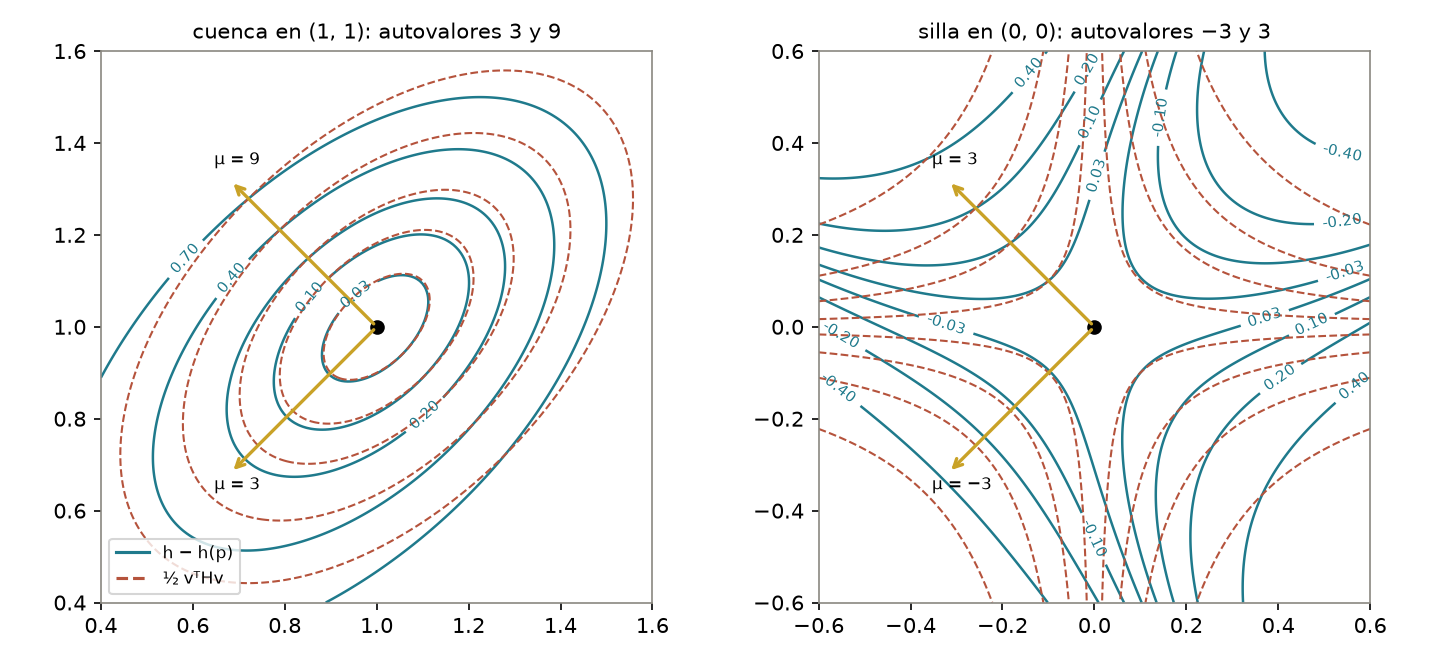
\includegraphics[width=.95\linewidth]{figuras/derivada/der_hessiana.png}
\caption{Curvas de nivel de \(h(x,y)-h(p)\) para \(h=x^3-3xy+y^3\) (teal) y de su aproximación
de segundo orden \(\tfrac12v^THv\) (óxido, punteadas), en los dos puntos críticos del
ejemplo~\ref{ej:der-hessiana}. Las flechas doradas son los autovectores de \(H\) con su
autovalor. Izquierda: cuenca en \((1,1)\), elipses. Derecha: silla en \((0,0)\), hipérbolas.
Cerca del punto las dos familias de curvas se confunden.}
\label{fig:der-hessiana}
\end{figure}

\subsection{Linealizar para resolver: el método de Newton}\label{sec:newton}

Suponé que desde un punto medís \(80\) m hasta el lugar que buscás y desde otro, \(60\) m. El
lugar está donde se cortan dos circunferencias. ¿Cómo se calcula ese corte? Con dos
circunferencias se puede despejar a mano, pero con mediciones de distinto tipo las ecuaciones
se vuelven inmanejables. La propuesta de Newton es otra: reemplazar cada curva por su recta
tangente, cortar rectas, que es fácil, y repetir desde el punto obtenido. Cortar dos distancias
(ubicar un punto por las distancias medidas desde dos puntos conocidos), cortar dos visuales
(ubicarlo por las direcciones en que se lo ve desde dos puntos conocidos; la visual es la línea
de mira) o calcular un punto por intersección inversa (ubicar dónde estamos parados midiendo
los ángulos hacia tres puntos conocidos) son
sistemas de ecuaciones no lineales. La idea del método de Newton es la del capítulo entero:
cerca de una aproximación \(x_k\), la que tenemos después de \(k\) pasos, reemplazar \(F\) por su
aproximación lineal y resolver el sistema \emph{lineal} para la corrección \(\delta\)
\[
  F(x_k)+J_F(x_k)\,\delta=0,\qquad x_{k+1}=x_k+\delta .
\]
En \(\R\) es el conocido \(x_{k+1}=x_k-f(x_k)/f'(x_k)\): cortar la recta tangente con el eje.
En el plano, cada ecuación se reemplaza por su recta tangente (la recta de nivel cero de la
forma afín, como en la sección~\ref{sec:niveles-nucleo}) y se cortan las dos rectas. Si
\(J_F\) es invertible en la solución y el arranque es bueno, el error de cada paso es
proporcional al cuadrado del error del paso anterior (convergencia cuadrática): cerca de la
solución, la cantidad de cifras correctas se duplica en cada iteración.

\begin{ejemplo}[Intersección de dos distancias por Newton]\label{ej:der-newton}
En un sistema local, desde \(A=(0,0)\) se midió \(80\) m y desde \(B=(100,0)\), \(60\) m, al
mismo punto \(X=(x,y)\), que está al norte de la base. Buscamos el cero de
\[
  F(x,y)=\begin{pmatrix}\lVert X-A\rVert-80\\ \lVert X-B\rVert-60\end{pmatrix},\qquad
  J_F=\begin{pmatrix}(X-A)^T/\lVert X-A\rVert\\ (X-B)^T/\lVert X-B\rVert\end{pmatrix}.
\]
Las filas de \(J_F\) son los versores que van de cada estación al punto: la primera fila del
\(J_{\operatorname{Pol}}\) del ejemplo~\ref{ej:der-dist-acimut}. Arrancamos de un croquis, \(x_0=(60,40)\).

\paragraph{Una iteración a mano.} Las distancias desde \(x_0\) son
\(\sqrt{60^2+40^2}=72{,}1110\) y \(\sqrt{40^2+40^2}=56{,}5685\), así que
\[
  F(x_0)=\begin{pmatrix}-7{,}8890\\-3{,}4315\end{pmatrix},\qquad
  J_F(x_0)=\begin{pmatrix}0{,}83205&0{,}55470\\-0{,}70711&0{,}70711\end{pmatrix},
  \qquad \det J_F=0{,}98058 .
\]
Resolviendo \(J_F\,\delta=-F\) se obtiene \(\delta=(3{,}7477;\ 8{,}6005)\) y
\(x_1=(63{,}7477;\ 48{,}6005)\). Desde \(x_1\) las distancias son \(80{,}1610\) y \(60{,}6320\):
los residuos pasaron de metros a decímetros.

\paragraph{Las siguientes.}
\begin{center}
\begin{tabular}{cccc}
\(k\) & \(x_k\) & \(y_k\) & distancia a la solución (m)\\\hline
\(0\) & \(60\) & \(40\) & \(8{,}94\)\\
\(1\) & \(63{,}747695\) & \(48{,}600509\) & \(0{,}651\)\\
\(2\) & \(64{,}001868\) & \(48{,}001649\) & \(2{,}49\cdot10^{-3}\)\\
\(3\) & \(64{,}000000\) & \(48{,}000000\) & \(5{,}14\cdot10^{-8}\)
\end{tabular}
\end{center}
La solución es \((64,48)\): \(64^2+48^2=80^2\) y \(36^2+48^2=60^2\). El error pasa de
\(0{,}651\) a \(0{,}0025\) y a \(5\cdot10^{-8}\): convergencia cuadrática. El determinante de \(J_F\) es el seno del ángulo entre las dos visuales; si el punto
estuviera casi alineado con \(A\) y \(B\), \(J_F\) sería casi singular, las rectas tangentes
casi paralelas y la intersección mal condicionada.
\end{ejemplo}

\begin{figure}[htbp]
\centering
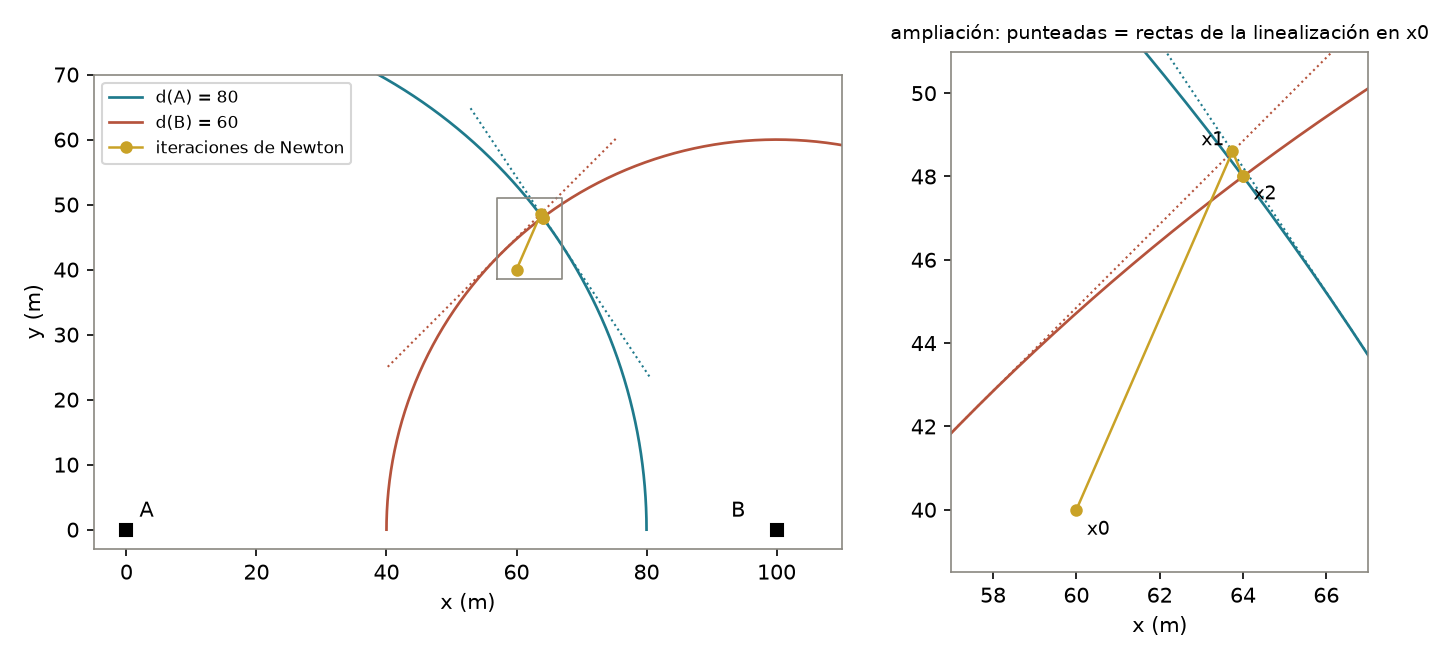
\includegraphics[width=.95\linewidth]{figuras/derivada/der_newton.png}
\caption{Las dos circunferencias del ejemplo~\ref{ej:der-newton} y las iteraciones de Newton
desde \(x_0=(60,40)\). Las rectas punteadas son las tangentes a cada circunferencia en el pie
de la visual desde \(x_0\): la linealización de \(F\) en \(x_0\). Su intersección es \(x_1\).
A la derecha, una ampliación.}
\label{fig:der-newton}
\end{figure}

Con más de dos distancias el sistema tiene más ecuaciones que incógnitas, y el paso de Newton
\(J_F\delta=-F\) no tiene solución exacta: se resuelve por cuadrados mínimos, buscando la
corrección que deja más chica la suma de los cuadrados de lo que no cierra, con la
pseudoinversa del capítulo~\ref{cap:inversas}. Ese es el método de Gauss--Newton, con el que
se resuelve el problema de la intersección de circunferencias del
capítulo~\ref{cap:cuatro-problemas}.

\subsection{La traza del jacobiano: divergencia de un campo de desplazamientos}

Imaginá que medís las mismas marcas del terreno hoy y dentro de unos años, y que entre una vez
y otra el suelo se movió unos centímetros, más en unos lugares que en otros. ¿Se estiró o se
comprimió el terreno alrededor de cada punto? Entre dos épocas, dos momentos en que se mide,
cada punto \(x\) del terreno se corre a \(x+\varepsilon u(x)\), donde
\(u\) es un campo de desplazamientos, la flecha que dice hacia dónde y cuánto se movió cada
punto, y \(\varepsilon\) indica que el corrimiento es chico.
El jacobiano de esa transformación es \(I+\varepsilon J\), con \(J\) el jacobiano de \(u\),
y el factor local de área es su determinante (sección~\ref{sec:metrica}). Por la
proposición~\ref{prop:traza-derivada-det}, \(\det(I+\varepsilon J)=1+\varepsilon
\operatorname{tr}J+O(\varepsilon^2)\), donde \(\operatorname{tr}J\) es la traza, la suma de la
diagonal, con el \(O(\varepsilon^2)\) en el sentido del
apéndice~\ref{ap:infinitesimales}. La traza de \(J\) es la \emph{divergencia} de \(u\),
\(\operatorname{div}u=\partial u_E/\partial E+\partial u_N/\partial N\), donde \(u_E\) y \(u_N\)
son las componentes este y norte del corrimiento. Cuando \(u\) es
afín, \(J\) es constante y el planteo se reduce al de la red deformada del
capítulo~\ref{cap:autovectores}: la divergencia es la dilatación de la
sección~\ref{sec:aplicacion-deformacion}, la parte simétrica de \(J\) es el tensor de
deformación (la matriz que dice cuánto se estira o se acorta cada dirección, sin contar el
giro) y la antisimétrica, un giro sin efecto sobre el área.

\begin{idea}[La divergencia mide cuánto se expande el terreno alrededor de un punto]
Divergencia positiva, el terreno se expande; negativa, se contrae; nula, solo se deforma o
gira sin cambiar de área.
\end{idea}

\subsection{Aplicación topográfica: cuánto error hereda un punto medido}\label{sec:aplicacion-radiacion}

Volvamos al temblor de la mano de \enquote{La idea}. Medimos un ángulo y una distancia desde un
punto conocido y con esos dos números calculamos otro punto. Cada medida viene con un pequeño
error: la distancia, de unos milímetros; el ángulo, de unos segundos de arco. ¿Cuánto error
hereda el punto calculado, y hacia qué lado?

\begin{idea}[Esto lo vas a usar en Topografía]
Ubicar un punto con una distancia y un ángulo medidos desde otro conocido es la función \(\operatorname{Rad}\)
de la sección~\ref{sec:inversa-local}. Calcular cuánto del error de las mediciones pasa a lo
calculado se llama \emph{propagación de errores}. El resultado se dibuja como una elipse
alrededor del punto, la \emph{elipse de error}, cuyo tamaño y forma dicen cuánto y hacia dónde
puede estar corrido.
\end{idea}

Desde un punto de coordenadas oficiales (sistema Gauss--Krüger, que divide el país en franjas
norte--sur numeradas; esta es la franja~5) \(E_0=5\,512\,340{,}00\) m,
\(N_0=6\,172\,480{,}00\) m se mide hasta otro punto la distancia \(d=1500{,}000\) m y la
dirección respecto del norte \(\mathrm{Az}=52^\circ30'00''\). Los números de las coordenadas son
largos porque se cuentan desde un origen lejano; lo que importa son las diferencias, no el
valor completo. El instrumento mide distancias con un desvío estándar de \(3\) mm \(+\ 2\) ppm y
direcciones con \(5''\). El \emph{desvío estándar}, que escribimos \(\sigma\), es el tamaño
típico del error de una medición; \(3\) mm \(+\ 2\) ppm quiere decir \(3\) mm fijos más \(2\) mm
por cada kilómetro medido (ppm: partes por millón). ¿Cuán bien queda determinado el punto?

\paragraph{El punto y su jacobiano.} Con \(\operatorname{Rad}(d,\mathrm{Az})=(E_0+d\sin\mathrm{Az},\
N_0+d\cos\mathrm{Az})\) el punto calculado es \(E=5\,513\,530{,}030\) m,
\(N=6\,173\,393{,}142\) m. Su jacobiano respecto de \((d,\mathrm{Az})\) es el \(J_{\operatorname{Rad}}\) del
ejemplo~\ref{ej:der-dist-acimut}:
\[
  J=\begin{pmatrix}\sin\mathrm{Az}&d\cos\mathrm{Az}\\ \cos\mathrm{Az}&-d\sin\mathrm{Az}\end{pmatrix}
  =\begin{pmatrix}0{,}793353&913{,}142\\0{,}608761&-1190{,}030\end{pmatrix}.
\]
La segunda columna está en metros por radián, así que el desvío del ángulo, \(\sigma_{\mathrm{Az}}\),
tiene que ir en
radianes: \(\sigma_{\mathrm{Az}}=5''=5\cdot\pi/(180\cdot3600)=2{,}424\cdot10^{-5}\) rad. El de la
distancia es \(\sigma_d=3+2\cdot1{,}5=6{,}0\) mm.

\paragraph{Cómo se reparte el error del punto.} Para describir el error de un punto no alcanza
con un número: hay que decir cuánto se equivoca en \(E\), cuánto en \(N\) y si los dos errores
tienden a ir juntos. Eso lo guarda una matriz simétrica, la \emph{matriz de covarianza}: en la
diagonal, los cuadrados de los desvíos de cada coordenada; fuera de ella, cuánto se acompañan
los dos errores. La escribimos \(\Sigma\) (sigma mayúscula, que acá no es una suma). Si los
errores de \(d\) y de \(\mathrm{Az}\) son chicos e
independientes, un error \(\varepsilon=(\varepsilon_d,\varepsilon_{\mathrm{Az}})\) en las
mediciones produce, a primer orden, el error \(J\varepsilon\) en el punto. Y esa matriz, para el error
\(J\varepsilon\), es \(J\,\Sigma\,J^T\) (si \(\Sigma=\mathrm{E}[\varepsilon\varepsilon^T]\),
entonces \(\mathrm{E}[J\varepsilon\varepsilon^TJ^T]=J\Sigma J^T\); \(\mathrm{E}[\cdot]\) es el
promedio sobre muchas repeticiones de la medición). Por lo tanto
\[
  \Sigma_{EN}=J\begin{pmatrix}\sigma_d^2&0\\0&\sigma_{\mathrm{Az}}^2\end{pmatrix}J^T
  =\begin{pmatrix}512{,}625&-621{,}150\\-621{,}150&845{,}499\end{pmatrix}\ \text{mm}^2 .
\]
Los desvíos de cada coordenada son \(\sigma_E=22{,}64\) mm y \(\sigma_N=29{,}08\) mm, con una
correlación de \(-0{,}9435\): los errores en \(E\) y en \(N\) no son independientes, aunque los
de \(d\) y \(\mathrm{Az}\) sí lo sean. La correlación es un número entre \(-1\) y \(1\) que dice
cuánto se acompañan dos errores; tan cerca de \(-1\), cuando uno sale por exceso el otro sale
casi siempre por defecto.

\paragraph{Semiejes y orientación.} Los autovalores de \(\Sigma_{EN}\) son \(1322{,}124\) y
\(36{,}000\) mm\(^2\); sus raíces, \(36{,}36\) mm y \(6{,}00\) mm, son los semiejes de la elipse
de error de un desvío, y los autovectores, con direcciones de \(142{,}50^\circ\) y
\(52{,}50^\circ\) respecto del norte,
sus direcciones (la lectura de una matriz así como elipse es la del
ejemplo~\ref{ej:svd-elipse-error}). El resultado tiene una lectura directa: las dos columnas de \(J\) son perpendiculares, una en la dirección de la visual y de
largo \(1\), la otra transversal y de largo \(d\). El semieje chico es \(\sigma_d\), sobre la
visual; el grande es \(d\,\sigma_{\mathrm{Az}}=1500\cdot2{,}424\cdot10^{-5}\) m \(=36{,}36\) mm,
perpendicular a ella. Es el temblor de la mano: un error de ángulo chico, multiplicado por un
brazo de un kilómetro y medio, corre el punto de costado varios centímetros.

\paragraph{Verificación por simulación.} Sorteamos \(10\,000\) mediciones con errores al
azar del tamaño de esos desvíos: la mayoría chicos, pocos grandes, repartidos como una campana
de Gauss. Para que cualquiera pueda repetir exactamente el mismo sorteo, lo fijamos con un número
de partida, la semilla \(2026\). Calculamos cada
punto con la \(\operatorname{Rad}\) exacta, con senos y cosenos, sin linealizar, y calculamos la misma matriz para
la nube de puntos, que llamamos \(\widehat\Sigma_{EN}\) (el sombrero indica que sale de los
datos simulados y no de la fórmula):
\[
  \widehat\Sigma_{EN}=\begin{pmatrix}516{,}783&-626{,}027\\-626{,}027&852{,}254\end{pmatrix}\ \text{mm}^2 .
\]
La diferencia relativa con \(J\Sigma J^T\) (en norma de Frobenius, la raíz de la suma de los
cuadrados de todas las entradas) es de \(0{,}79\)\,\%, del
orden del error de muestreo con \(10\,000\) puntos; los semiejes empíricos son \(36{,}51\) mm y
\(6{,}03\) mm. Dentro de la elipse de un desvío cae el \(38{,}33\)\,\% de los puntos y dentro de
la del \(95\)\,\% (la agrandada para que, en teoría, contenga el \(95\)\,\% de los puntos), el
\(94{,}95\)\,\%. La linealización en sí no aporta error visible: sobre la
misma muestra, la máxima diferencia entre \(\operatorname{Rad}\) exacta y \(\operatorname{Rad}(p)+J\varepsilon\) es de
\(5{,}17\) micrómetros, porque los errores angulares son de \(10^{-5}\) rad y el término de
segundo orden es del orden de \(d\,\sigma_{\mathrm{Az}}^2\).

\begin{figure}[htbp]
\centering
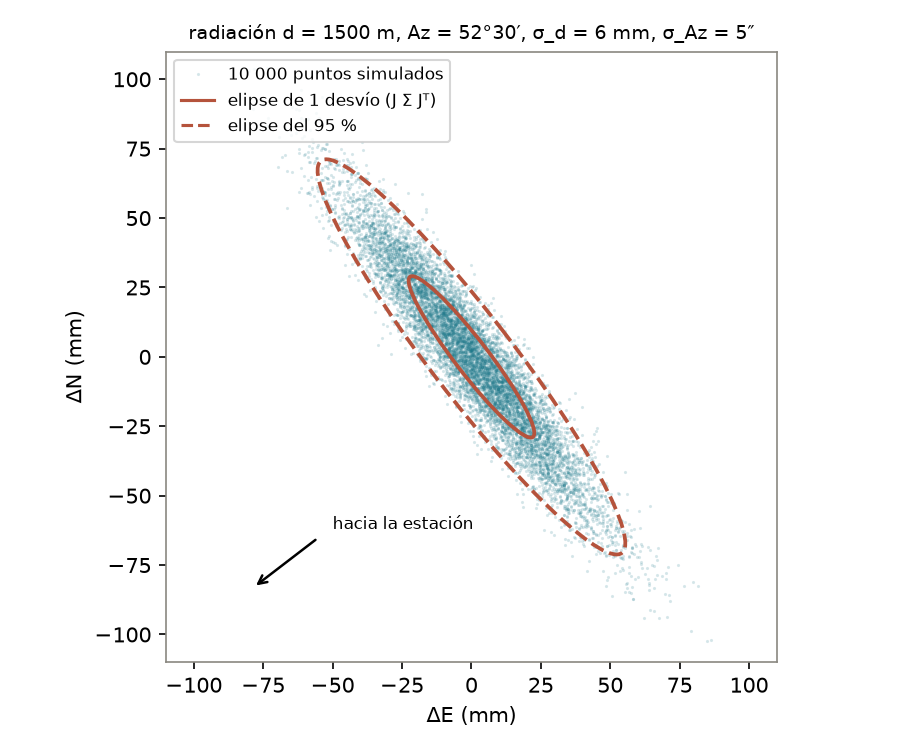
\includegraphics[width=.66\linewidth]{figuras/derivada/der_radiacion.png}
\caption{Los \(10\,000\) puntos simulados alrededor del punto radiado (diferencias en mm) y las
elipses de un desvío y del \(95\)\,\% que da \(J\,\Sigma\,J^T\). El eje mayor, de \(36{,}36\) mm,
es perpendicular a la visual; el menor, de \(6{,}00\) mm, está sobre ella.}
\label{fig:der-radiacion}
\end{figure}

\paragraph{El error transversal domina.} Con los mismos instrumentos, para distintas
distancias:
\begin{center}
\begin{tabular}{cccc}
\(d\) (m) & \(\sigma_d\) (mm) & \(d\,\sigma_{\mathrm{Az}}\) (mm) & cociente\\\hline
\(500\) & \(4{,}0\) & \(12{,}1\) & \(3{,}03\)\\
\(1000\) & \(5{,}0\) & \(24{,}2\) & \(4{,}85\)\\
\(1500\) & \(6{,}0\) & \(36{,}4\) & \(6{,}06\)\\
\(2000\) & \(7{,}0\) & \(48{,}5\) & \(6{,}93\)
\end{tabular}
\end{center}
El error sobre la visual crece apenas \(2\) mm por kilómetro; el transversal, \(24{,}2\) mm por
kilómetro. Los dos se igualan cuando \(d\,\sigma_{\mathrm{Az}}=3\text{ mm}+2\cdot10^{-6}d\),
es decir en \(d\approx135\) m; para puntos más lejanos la elipse es cada vez más alargada y
la calidad del punto depende sobre todo de la del ángulo. Por eso, para mejorar un punto lejano,
conviene mejorar el ángulo antes que la distancia.

\section{Ejercicios con solución}

\begin{ejercicio}\label{ex:der-jacobiano}
Sea \(F(x,y)=(x^2-y,\ xy)\). Escribí su jacobiano en \((2,1)\), usalo para aproximar
\(F(2{,}1;\ 0{,}9)\) y compará con el valor exacto. ¿Cuánto vale el factor local de área en
ese punto?
\end{ejercicio}
\solucion{\(J=\left(\begin{smallmatrix}2x&-1\\y&x\end{smallmatrix}\right)
=\left(\begin{smallmatrix}4&-1\\1&2\end{smallmatrix}\right)\) en \((2,1)\), donde \(F=(3,2)\).
Con \(v=(0{,}1;\ -0{,}1)\), \(Jv=(0{,}5;\ -0{,}1)\) y la aproximación es \((3{,}5;\ 1{,}9)\);
el valor exacto es \((2{,}1^2-0{,}9;\ 2{,}1\cdot0{,}9)=(3{,}51;\ 1{,}89)\). Las diferencias,
\(0{,}01\) y \(-0{,}01\), son de segundo orden (\(h^2\) y \(hk\)). El factor de área es
\(\det J=9\): cerca de \((2,1)\) las áreas se multiplican por \(9\), sin cambio de orientación.}

\begin{ejercicio}\label{ex:der-cadena}
Sea \(h(x,y)=xy\) y \((x,y)=P(r,\theta)=(r\cos\theta,r\sin\theta)\). Calculá la fila de
\(h\circ P\) en \(r=2\), \(\theta=30^\circ\) con la regla de la cadena, usando el jacobiano del
ejemplo~\ref{ej:der-polares}, y comprobala derivando directamente
\(h(P(r,\theta))=\tfrac12r^2\sin2\theta\).
\end{ejercicio}
\solucion{En \(P(2,30^\circ)=(1{,}732;\ 1)\) la fila de \(h\) es \((y,x)=(1;\ 1{,}732)\). Por
la regla de la cadena,
\((1;\ 1{,}732)\left(\begin{smallmatrix}0{,}866&-1\\0{,}5&1{,}732\end{smallmatrix}\right)
=(0{,}866+0{,}866;\ -1+3)=(1{,}732;\ 2)\). Directamente:
\(\partial_r=r\sin2\theta=2\sin60^\circ=1{,}732\) y \(\partial_\theta=r^2\cos2\theta=4\cdot0{,}5=2\).
La fila se multiplica por \(J\) a la derecha, como toda forma lineal.}

\begin{ejercicio}\label{ex:der-hessiana}
Un relieve se modela cerca del origen como \(h(x,y)=100-x^2+xy-2y^2\) (en metros, con \(x,y\)
en unidades de \(10\) m). Verificá que el origen es punto crítico, clasificalo por los
autovalores de la hessiana e indicá las direcciones de curvatura máxima y mínima.
\end{ejercicio}
\solucion{El gradiente, \((-2x+y,\ x-4y)\), se anula en \((0,0)\). La hessiana es
\(H=\left(\begin{smallmatrix}-2&1\\1&-4\end{smallmatrix}\right)\), con traza \(-6\) y
determinante \(7\); sus autovalores son \(-3\pm\sqrt2\): \(-4{,}414\) y \(-1{,}586\).
Los dos negativos: el origen es una cima, con \(h=100\). La bajada más brusca va según el
autovector de \(-4{,}414\), \((0{,}383;\ -0{,}924)\) (casi en la dirección \(y\)), y la más
suave según el de \(-1{,}586\), \((0{,}924;\ 0{,}383)\). Como \(h\) es cuadrática, la fórmula de
segundo orden es exacta: con \(v=(1,1)\), \(\tfrac12v^THv=-2\) y \(h(1,1)=98\).}

\begin{ejercicio}\label{ex:der-newton}
Desde \(A=(0,0)\) se midió \(30\) m y desde \(B=(50,0)\), \(40\) m al mismo punto, ubicado al
norte de la base. Partiendo de \(x_0=(20,20)\), hacé una iteración de Newton a mano con la
\(F\) del ejemplo~\ref{ej:der-newton} y compará con la solución exacta.
\end{ejercicio}
\solucion{Desde \(x_0\) las distancias son \(28{,}2843\) y \(36{,}0555\), y
\(F(x_0)=(-1{,}7157;\ -3{,}9445)\). Las filas de \(J_F\) son los versores desde cada estación:
\(J_F=\left(\begin{smallmatrix}0{,}70711&0{,}70711\\-0{,}83205&0{,}55470\end{smallmatrix}\right)\),
con \(\det J_F=0{,}98058\). Resolviendo \(J_F\delta=-F\): \(\delta=(-1{,}8738;\ 4{,}3003)\) y
\(x_1=(18{,}1262;\ 24{,}3003)\). La solución exacta es \((18,24)\) (\(18^2+24^2=30^2\),
\(32^2+24^2=40^2\)); el error pasa de \(4{,}47\) m a \(0{,}326\) m, y una segunda iteración da
\((17{,}9991;\ 24{,}0008)\), a \(1{,}25\) mm.}

\begin{ejercicio}\label{ex:der-radiacion}
Se radia un punto con \(d=800\) m y \(\mathrm{Az}=300^\circ\), con \(\sigma_d=3\) mm \(+\ 2\) ppm y
\(\sigma_{\mathrm{Az}}=10''\). Calculá \(\Sigma_{EN}=J\,\mathrm{diag}(\sigma_d^2,\sigma_{\mathrm{Az}}^2)\,J^T\),
los semiejes de la elipse de un desvío y sus acimutes.
\end{ejercicio}
\solucion{\(\sigma_d=3+1{,}6=4{,}6\) mm y \(\sigma_{\mathrm{Az}}=10''=4{,}848\cdot10^{-5}\) rad,
de modo que \(d\,\sigma_{\mathrm{Az}}=38{,}79\) mm. Con \(\sin300^\circ=-0{,}866\) y
\(\cos300^\circ=0{,}5\),
\(J=\left(\begin{smallmatrix}-0{,}866&400\\0{,}5&692{,}820\end{smallmatrix}\right)\) y
\(\Sigma_{EN}=\left(\begin{smallmatrix}391{,}941&642{,}211\\642{,}211&1133{,}503\end{smallmatrix}\right)\)
mm\(^2\). Como las columnas de \(J\) son perpendiculares, los semiejes son \(\sigma_d=4{,}60\) mm,
sobre la visual (acimut \(120^\circ\), o \(300^\circ\)), y \(d\,\sigma_{\mathrm{Az}}=38{,}79\) mm,
transversal (acimut \(30^\circ\), o \(210^\circ\)): la elipse es más de ocho veces más larga que ancha.}
